%% The '3p' and 'times' class options of elsarticle are used for Elsevier CRC
%% Add the 'procedia' option to approximate to the Word template
%\documentclass[3p,times,procedia]{elsarticle}
\documentclass[3p,times]{elsarticle}

%% The `ecrc' package must be called to make the CRC functionality available
\usepackage{ecrc}
\usepackage{color,soul}
\usepackage{multirow}
\usepackage{booktabs}
\graphicspath{{images/}}

\usepackage{lscape}


\volume{00}
\firstpage{1}
\journalname{Forest ecology and management}
\runauth{Gilles A. et al.}

%% Give the abbreviation of the Journal. %% A user-supplied logo with the name <\jid>logo.pdf will be inserted if present.
\jid{feam}
\jnltitlelogo{Forest ecology and management}
\CopyrightLine{2022}{Published by Elsevier Ltd.}

\usepackage{amssymb}
\usepackage{lineno}

\usepackage{hyperref}
\usepackage{subfig}
\usepackage[export]{adjustbox}

% if you have landscape tables
%\usepackage[figuresright]{rotating}
% add words to TeX's hyphenation exception list
%\hyphenation{author another created financial paper re-commend-ed Post-Script}

\begin{document}

\begin{frontmatter}

%% Title, authors and addresses

%% use the tnoteref command within \title for footnotes;
%% use the tnotetext command for the associated footnote;
%% use the fnref command within \author or \address for footnotes;
%% use the fntext command for the associated footnote;
%% use the corref command within \author for corresponding author footnotes;
%% use the cortext command for the associated footnote;
%% use the ead command for the email address,
%% and the form \ead[url] for the home page:
%%
%% \title{Title\tnoteref{label1}}
%% \tnotetext[label1]{}
%% \author[label1,label2]{<author name>}
\author[label2]{Gilles Arthur}
\ead{tonemail}
\author[label2]{Lisein Jonathan}
%\ead{liseinjon@hotmail.com}
\author[label2]{Claessens Hugues}

%% \ead[url]{home page}
\fntext[label2]{Liège University - Faculty of Gembloux Agro-Bio Tech - unit of forest ressources managment}
%\fntext[label1]{Forêt.Nature asbl}
%\cortext[cor1]{}
%% \address{Address\fnref{label3}}
%% \fntext[label3]{}

\dochead{Original research papers}
%% Use \dochead if there is an article header, e.g. \dochead{Short communication}
%% \dochead can also be used to include a conference title, if directed by the editors
%% e.g. \dochead{17th International Conference on Dynamical Processes in Excited States of Solids}

%pdftotext 2021-phytoSpy.pdf - | tr -d '.' | wc -w pour le nombre de mot

\title{Bark beetle infection of spruce differs between Belgium and north France : a remote sensing analysis of 2016-2021 dieback}

\begin{abstract}

\end{abstract}

\begin{keyword}
% nutrient regime \sep moisture regime
\end{keyword}

\end{frontmatter}

\linenumbers

\pagebreak
\section{Introduction}

\begin{itemize}
	\item Aire de répartition de l'épicéa
	\item Scolyte description générale, plus précision typographe chalcographe
	\item Evolution des dégats lié au scolyte dans le monde
	\item Début de la crise en Wallonie + Vosges en 2018
	\item Objectif de l'article: caractérisation des attaque de scolytes en Wallonie et dans les Vosges selon deux variables environnementales +paramètres macro 
\end{itemize}

\section{Matériel et méthode}

\subsection{Description zone de la Zone d'étude}

\begin{itemize}
	\item Description zone d'étude générale + tuile S2 traitées (figure: \ref{fig:rep_vosg}) 
	\item Description générale de la forêt wallonne 
	\item Description de la pessière wallonne 
	\item Description générale de la foret vosgienne 
	\item Description de la pessière vosgienne
	\item Comparaison Température et précipitation vosges et Wallonie entre moyenne trentenaire et données pour l'année 2018 (figure \ref{fig:diagOT})
	
\end{itemize}



\subsection{Données de MNT et de Sous-secteurs Radiatif}

\begin{itemize}
	\item Provenance des données de MNT
	\item Méthodologie de calcul des sous-secteur radiatif.
\end{itemize}


\subsection{Mapping of spruce dieback and mortality by analysis of sentinel-2 time-serie}


The European Union’s earth observation programme, with its satellite twin constellation Sentinel-2A and Sentinel-2B, provides free earth imagery with a high revisit time. 
Sentinel-2 (S2) satellites carry multispectral sensor with a ground resolution up to 10 m. 
S2 imagery have been intensively used recently for forestry purpose, including for the monitoring of bark beetle outbreaks. 
Low and Koukal \citep{low_phenology_2020} have modelled phenology courses of vegetation indices to detect forest disturbances. 
They have properly mapped Bark beetle infestation in Austrian spruce stands.
Ali \textit{et al.} \citep{ali_canopy_2021} have used multi-years time series remote sensing data in order to detect early bark beetle infestation in Germany. 
They have highlighted the potential of S2 data for the production of reliable infestation maps.
Barta \textit{et al.} \citep{barta_early_2021} have studied spectral trajectories of nine bands and six vegetation indices from S2 imagery for the 2018 vegetation season. 
They have confirmed the superiority of multi-date data for the classification by Random Forest of infested stands in the Czech Republic.

In this present research, the detection of bark beetle infestation is realized by using dense time series of S2 imagery following the methodology developped by Dutrieux \textit{et al.} \citep{dutrieux_package_2021}.
Vegetation changes are tracked by means of a phenology metric, the \textit{SWIR Continuum Removal} ($SWIR_{CR}$) indice.
All S2 acquisitions are used in the analyses, provided that the cloud couver do not excess 35 percent.  Bottom Of Atmosphere reflectance images (L2A product) are downloaded from the Theia data cluster \citep{theia_team_value-added_nodate} for all the 6 granules, which are tiles of 100km x 100km, that covers Wallonia. 
For north France, one single granule covers the Vosges mountains.
The $SWIR_{CR}$ is based on three spectral bands, the near-infrared, the shortwave infrared 1 band and the shortwave infrared 2, and is sensitive to the foliage water content (figure \ref{fig:harmo}).
Seasonal variation of $SWIR_{CR}$ for healthy stand is modelled and a bark beetle attack is detected if the observations deviates from the healthy phenology trajectory. 
Figure \ref{fig:harmo} illustrates a time-serie of $SWIR_{CR}$ observations (grey dots) for one pixel. 
In 2018, the observations goes beyond the threshold represented by the purple-dashed line, which shows that the spruce stand suffer from a serious stress induced by a bark beetle attack.
A bark beetle outbreak is confirmed as soon as $SWIR_{CR}$ vegetation indice show a stress for at least three consecutive times.
In parallel to the detection of bark beetle stress, stand cutting and thinning are subject of particular attention. 
Bare soil is detected by using a combination of red, green and shortwave infrared reflectance values.
Cutting are thus taken into account and are classified either as normal harvest cutting or as sanitary thinning based on the health status prior to the cutting.
The analysis of image time-serie is thus quite straightforward and is performed individually pixel per pixel starting from the 2016 year, which is the beginning of S2 acquisitions. 
The dense time-serie covers the 2016-2021 period and count a minimum of 180 acquistion dates. 
The health status is summarized in annual health maps by means of four classes ; healthy, bark beetle attached, cutted and sanitary thinning.

\begin{figure}
	\centering
	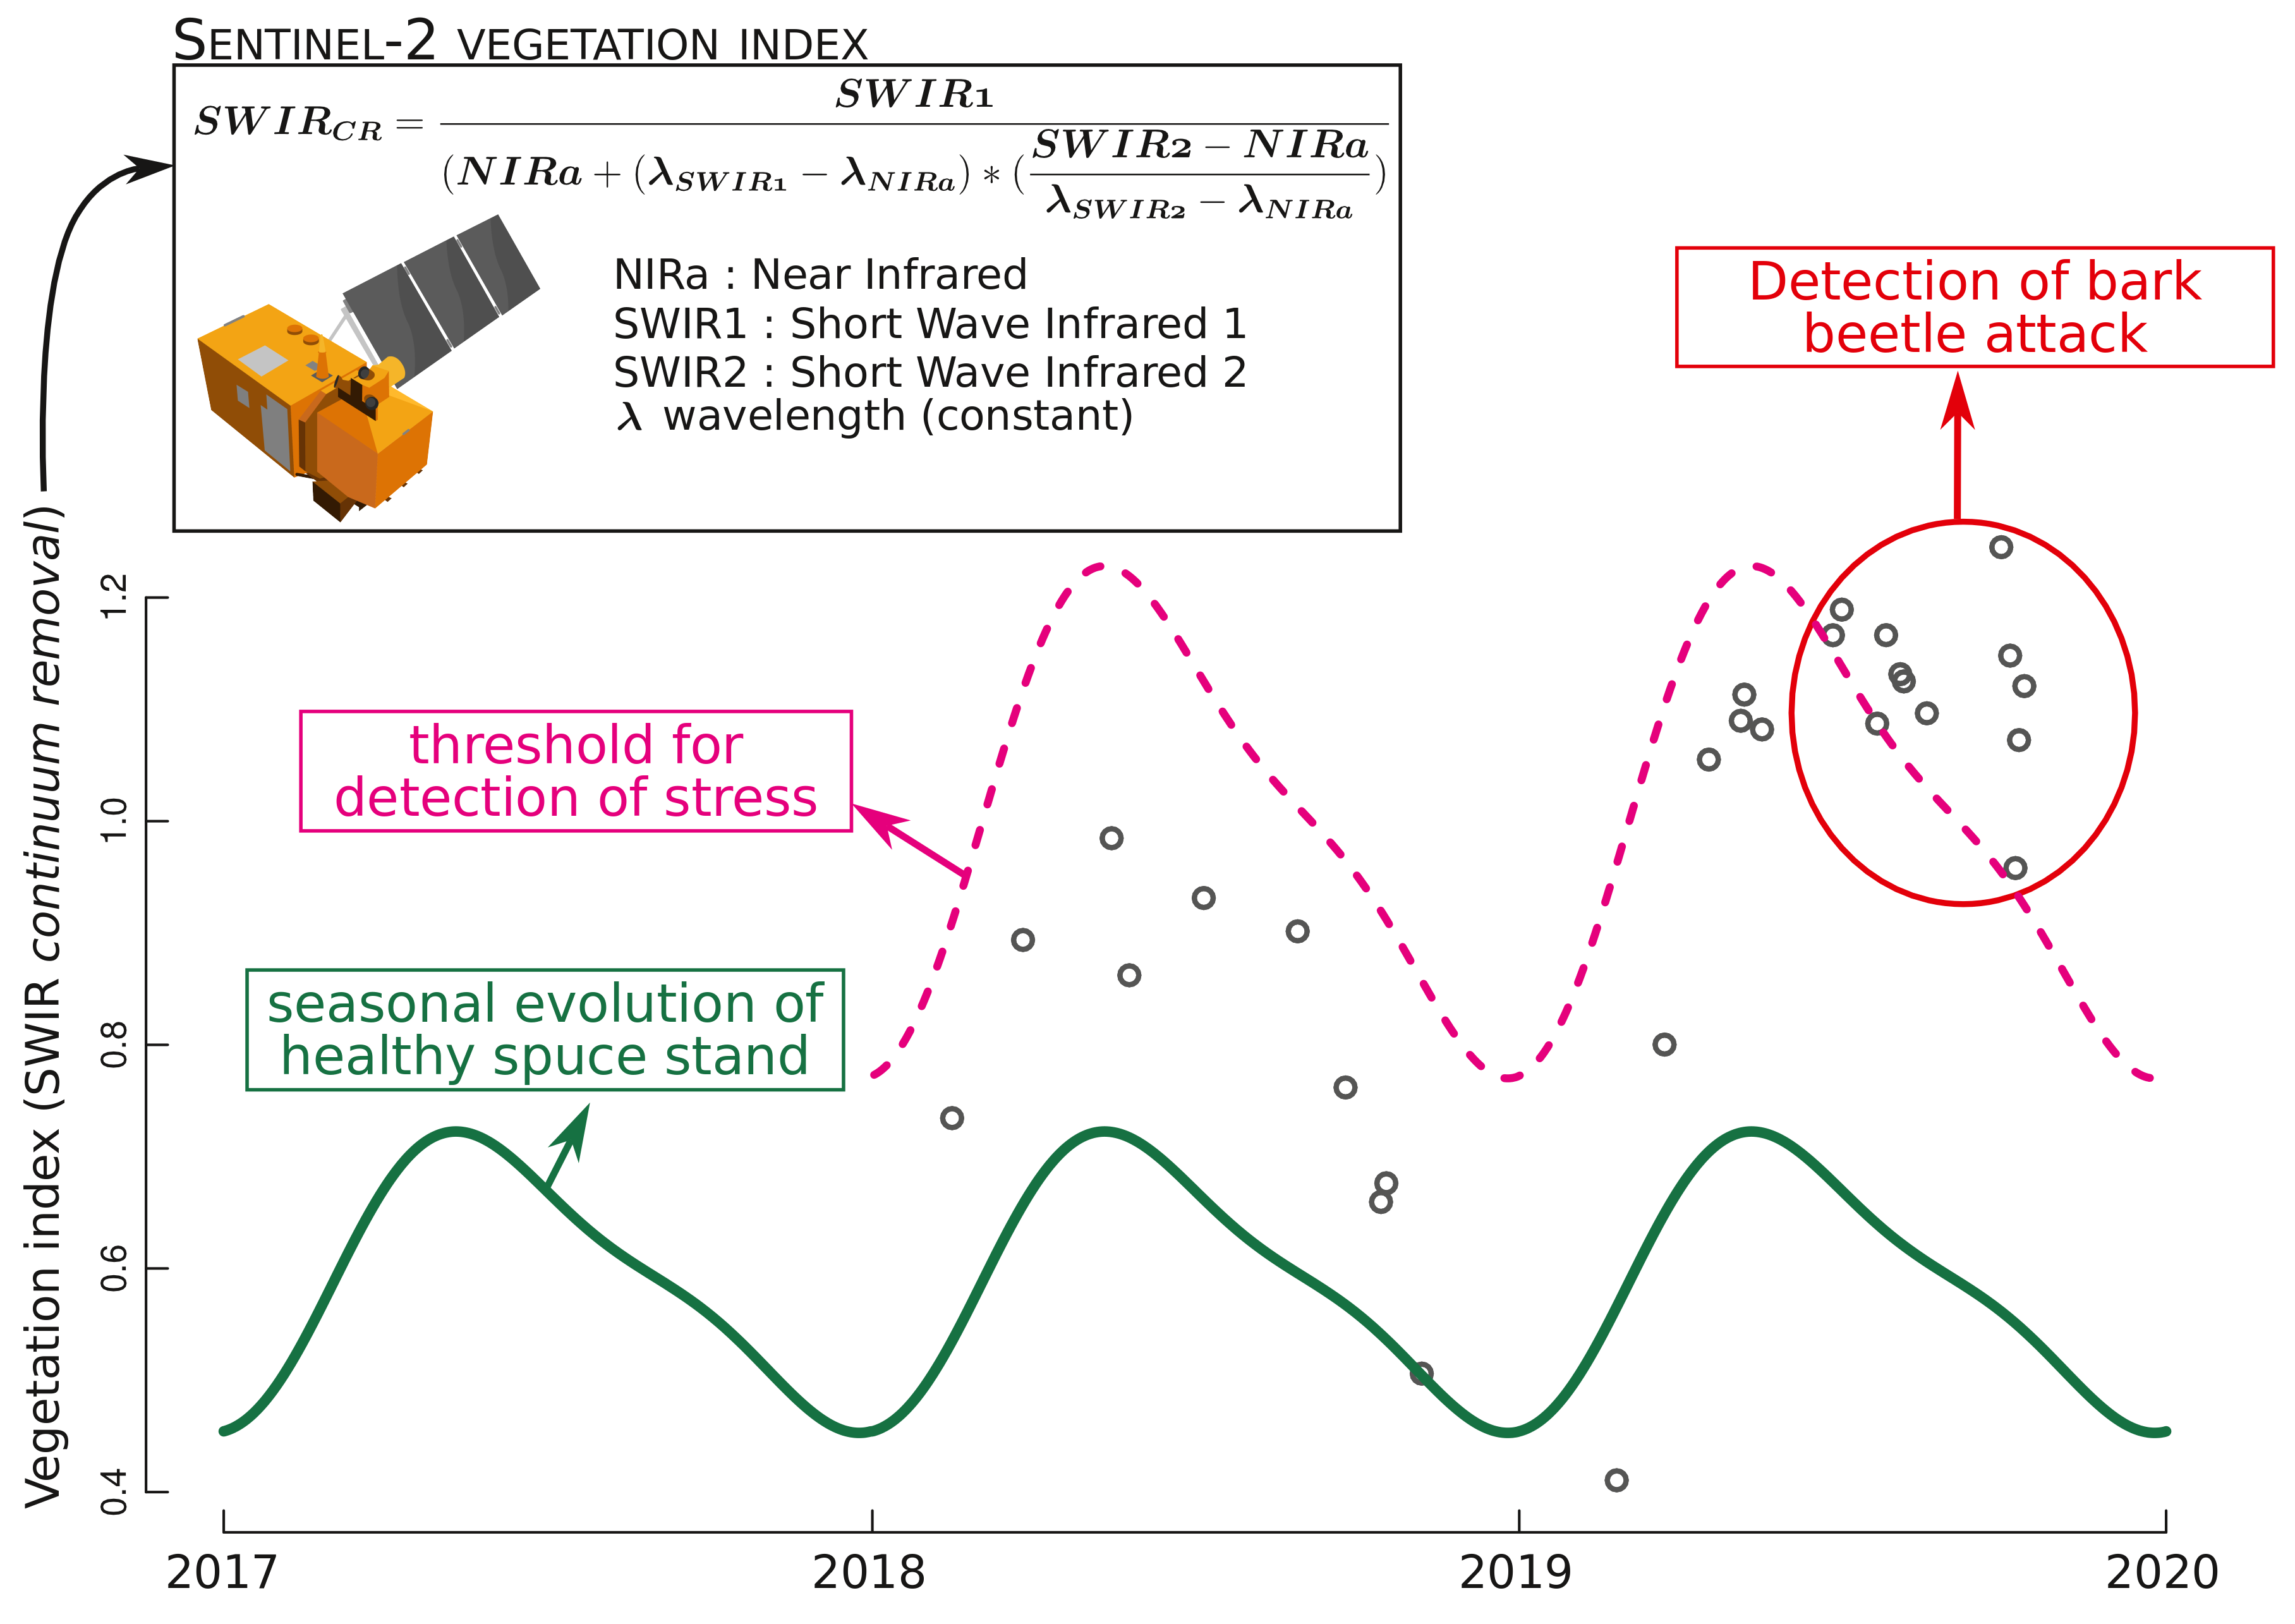
\includegraphics[width=\textwidth]{fctHarmo.png}
	\caption{Bark beetle infestation map are computed by detecting change in the $SWIR_{CR}$ phenology metric. The \textit{SWIR Continuum Removal} is computed using three bands from Sentinel-2 imagery for every single acquisition date and his value is compared to a threshold (purple dashed line) in order to detect vegetation stress. If a stress is detected three consecutive times, we assume that a bark beetle infection occured.}
	\label{fig:harmo}
\end{figure}

Our approach of bark beetle detection is only suitable for spruce, as it is closely related to the phenological course of healthy spruce forest.
An essential prerequisite is thus to have a proper mapping of spruce stands.
For the south of Belgium, we use existing reliable composition maps \citep{bolyn_forest_2018} computed from remote sensing data in order to restrict our analysis to spruces.
In Vosges mountains, the composition map comes from the French Mapping agency (Forest BD version 2). 
Composition of forest stand is determined by photointerpretation and forest stands identifyed as "spruce or fir" serve as starting point to limit our analysis.
Time series are a convenient means to track phenology changes. 
More broadly than the dectection of bark beetle infestion, phenology courses are highly suitable for forest tree species discrimination \citep{lisein_discrimination_2015,grabska_forest_2019,ma_tree_2021}.
We have used S2 spectral bands courses along the vegetation season to refine the determination of species present in the area interpreted as "spruce or fir" in Vosges.
The objective is to identify and remove every area that are not spruce stand, as pixels located on others species than spruce are likely to be wrongly detected as a bark beetle attack.
All S2 spectral bands were first summarized for each of the four trimesters of the year, by simply averaging all observations occuring during the trimester.
Then, a Random Forest algorithm was trained on these synthetic intra-annual time serie to discriminate spruce from non-spruce pixels, based on a training set of observation from Belgium \citep{bolyn_forest_2018}.
Eventually, this Random Forest classifier was applied on "spruce and fir" area of Vosges and bark beetle detection was carried on only for pixels detected as spruce. 






\subsection{Analyse stat}
\begin{itemize}
	\item test de student 
\end{itemize}

\section{résultats}

\subsection{ Altitude vs probabilité de présence de scolyte}



\begin{itemize}
	\item Description figure \ref{fig:sco_alti}
	\item Wallonie: Diminution de la probabilité de présence de scolyte avec l'augmentation de l'altitude 
	\item Vosges pas de relation clair avec l'altitude. Cependant, les classes d'altitude 2, 11 et 12 semblent + touchées que les autres classes d'altitude
	
	\item Wallonie + Vosges: Augmentation de la probabilité de présence de scolyte avec le temps quelque soit la classe d'altitude.
\end{itemize}



\subsection{Sous-secteur radiatif vs probabilité de présence de scolyte}


\begin{itemize}
	\item Description figure \ref{fig:ss_wall} 
	\item Wallonie: Différences significative entre les différents sous secteurs. Les sous secteur froid sont  plus touchés que les sous secteur chaud et les plateaux. Les plateaux sont moins touché en Wallonie.
	\item Vosges: pas de différence significative entre les sous secteurs ( \ref{fig:ss_vosg})
	
\end{itemize}

%sous-secteur
%graphe + descruipton


\section{Discussion}

\subsection{Différence entre Vosges et Wallonie}
\begin{itemize}
	\item Différence climat (Climat semicontinental/montagnard vs climat tempéré océanique)
	\item Différence sylvicole ( Wallonie futaie régulière exploitable vs Vosges peuplement + mélangé et moins exploitable en haute altitude)
	\item Sommet des vosges epicéas endémiques vs épicéas en plantations (résilience peuplement )
	
\end{itemize}

\subsection{Facteur déterminant l'attaque par l'épicéa ou le scolyte}

\begin{itemize}
	\item Discussion généralisation de modèle scolyte/ dépérissement des épicéas
	\item est ce la Biologie du scolyte/ ou le stress de l'épicéa qui conditionne le dépérissement massif ?
	
\end{itemize}

\section{Conclusion}

Dépérissement différents pour les Vosges et la Wallonie.

\section{Figure}

\begin{figure} [htbp] 
	\centering
	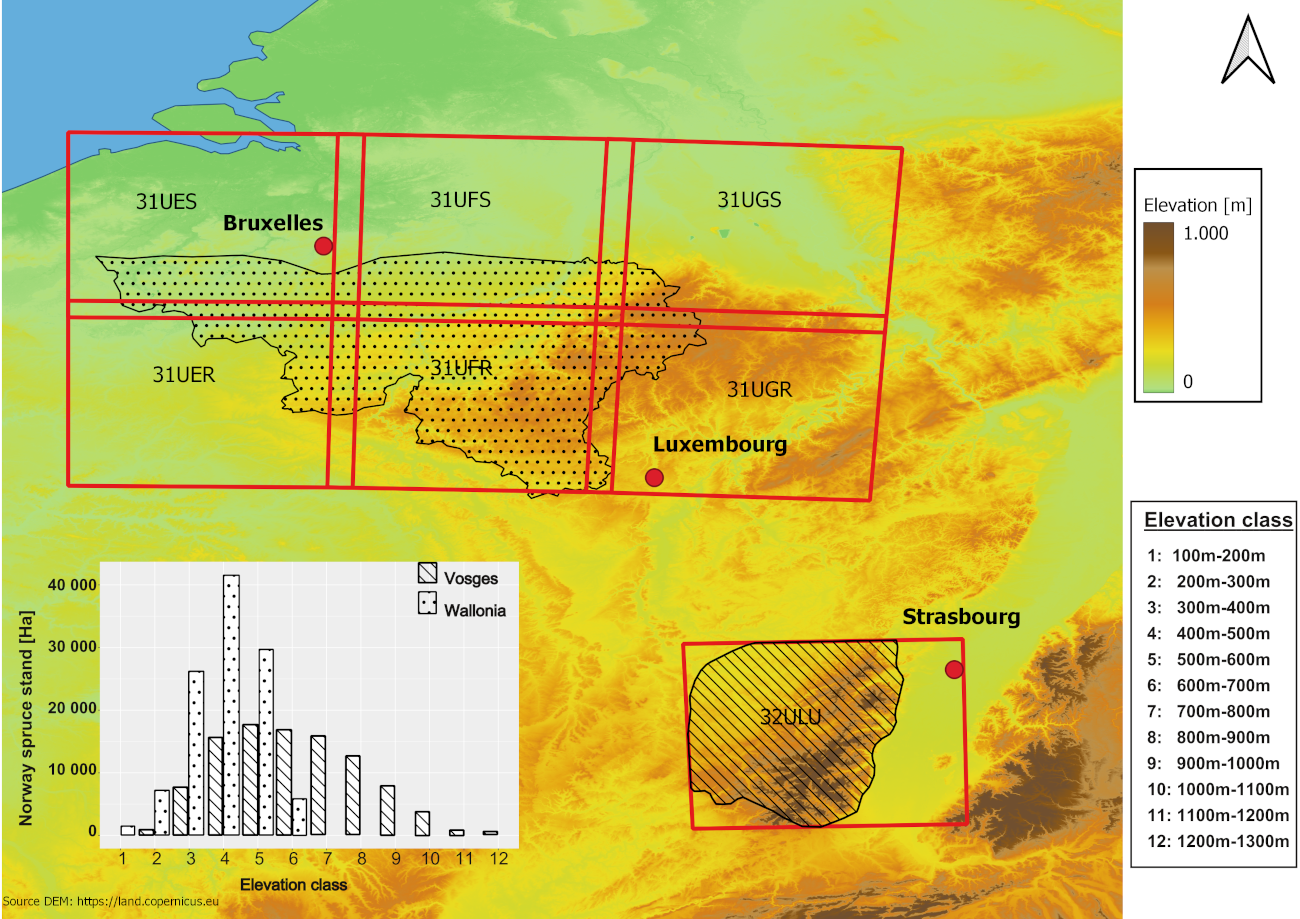
\includegraphics[width=1\textwidth]{waql.png}
	\caption{Zones d'études avec le MNT (XXX) et les tuiles du satellite Sentinelle 2 employées(XXX légende carré rouge).}
	\label{fig:situ}
\end{figure}


\begin{figure} [htbp] 
	\centering
	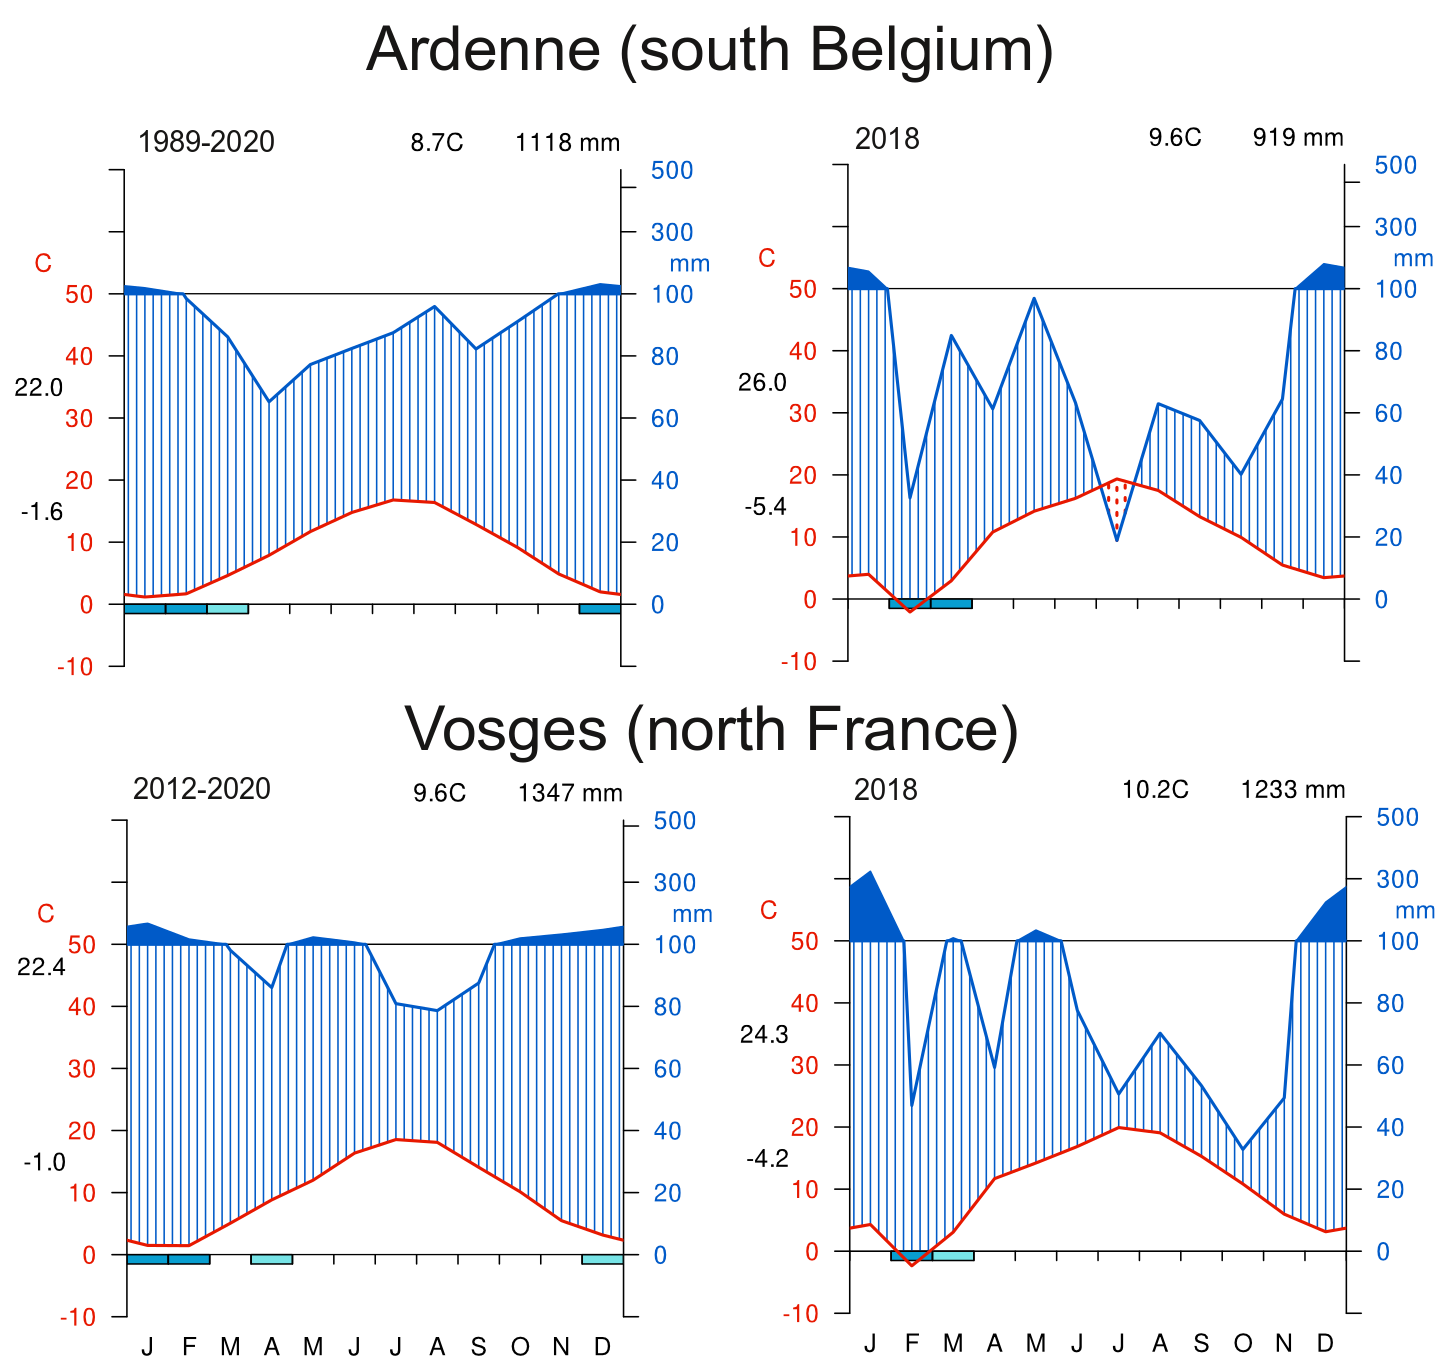
\includegraphics[width=1\textwidth]{diagrammeOT-page001.png}
	\caption{Walter and Lieth climatic diagram comparison for Ardenne (up) and Vosges (down). Left diagram show the average recent climate, and rigth one illustrates the year of 2018.}
	\label{fig:diagOT}
\end{figure}


\begin{figure} [htbp] 
		\centering
		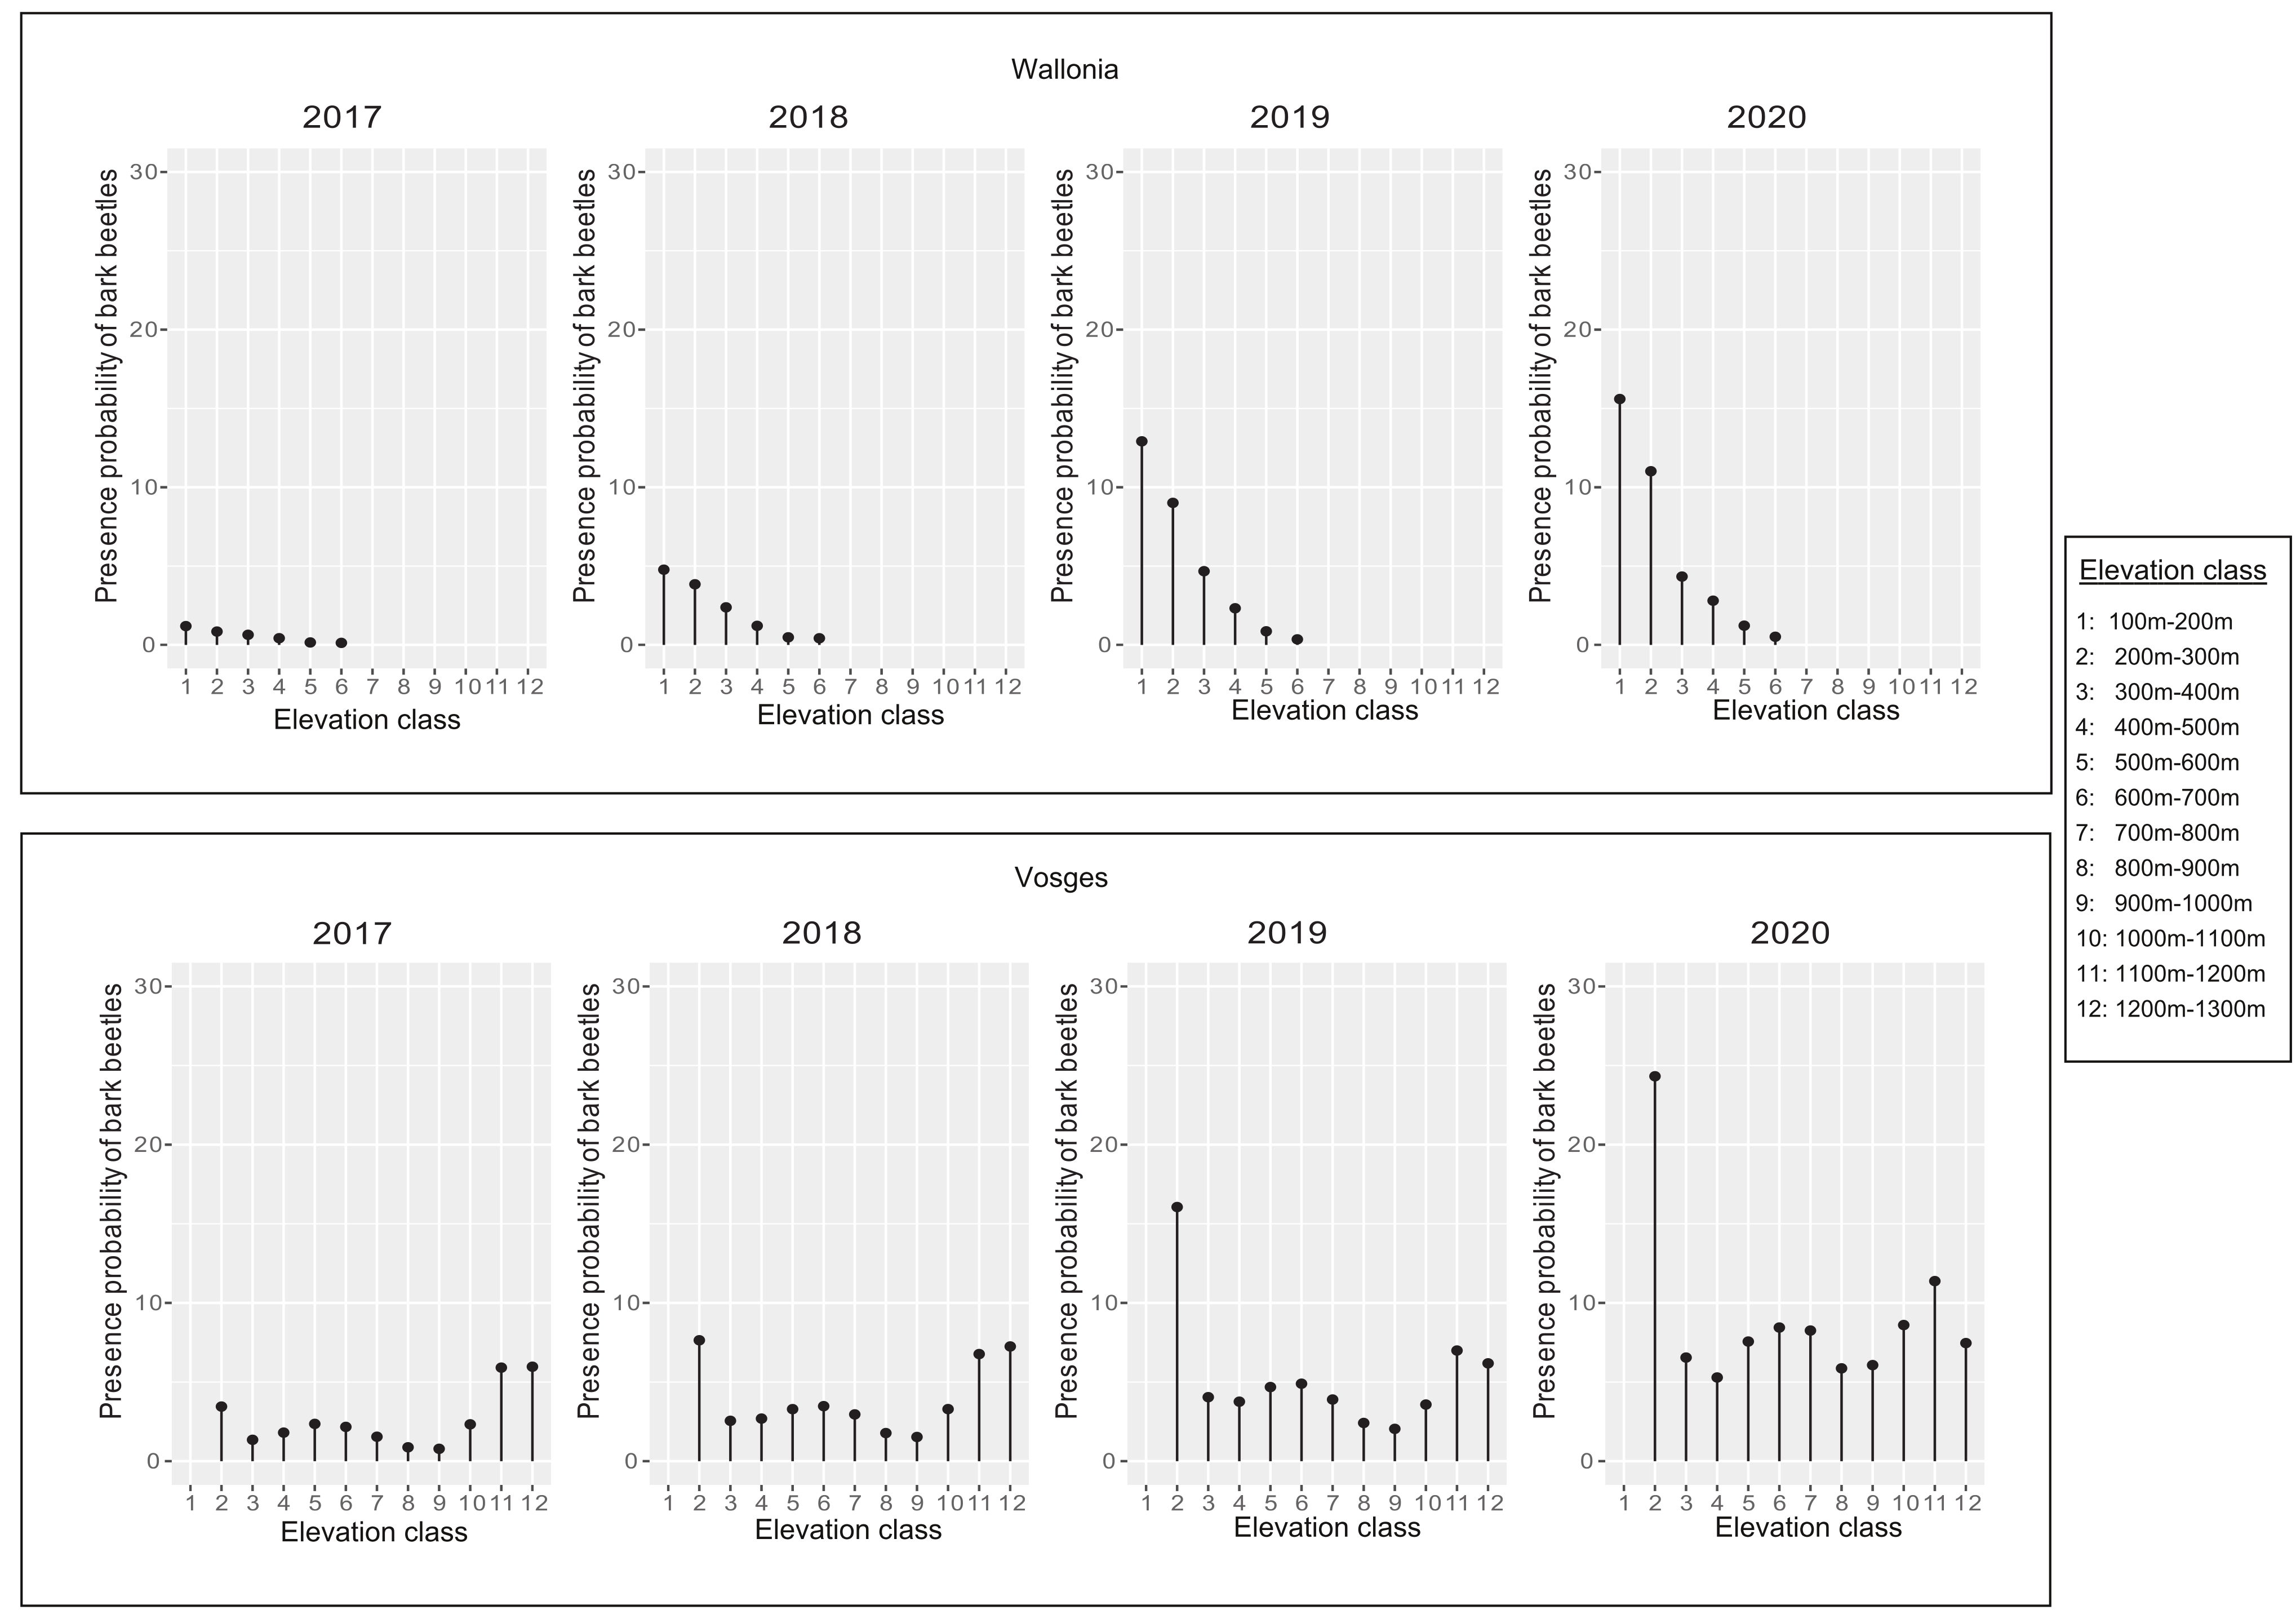
\includegraphics[width=1\textwidth]{Wall_vs_vosges.png}
		\caption{Probabilité de présence de scolyte en fonction de l'altitude pour la Wallonie et les Vosges}
		\label{fig:sco_alti}
\end{figure}
	

\begin{figure}[htbp]
	\begin{minipage}[b]{1 \linewidth}
		\centering
	%	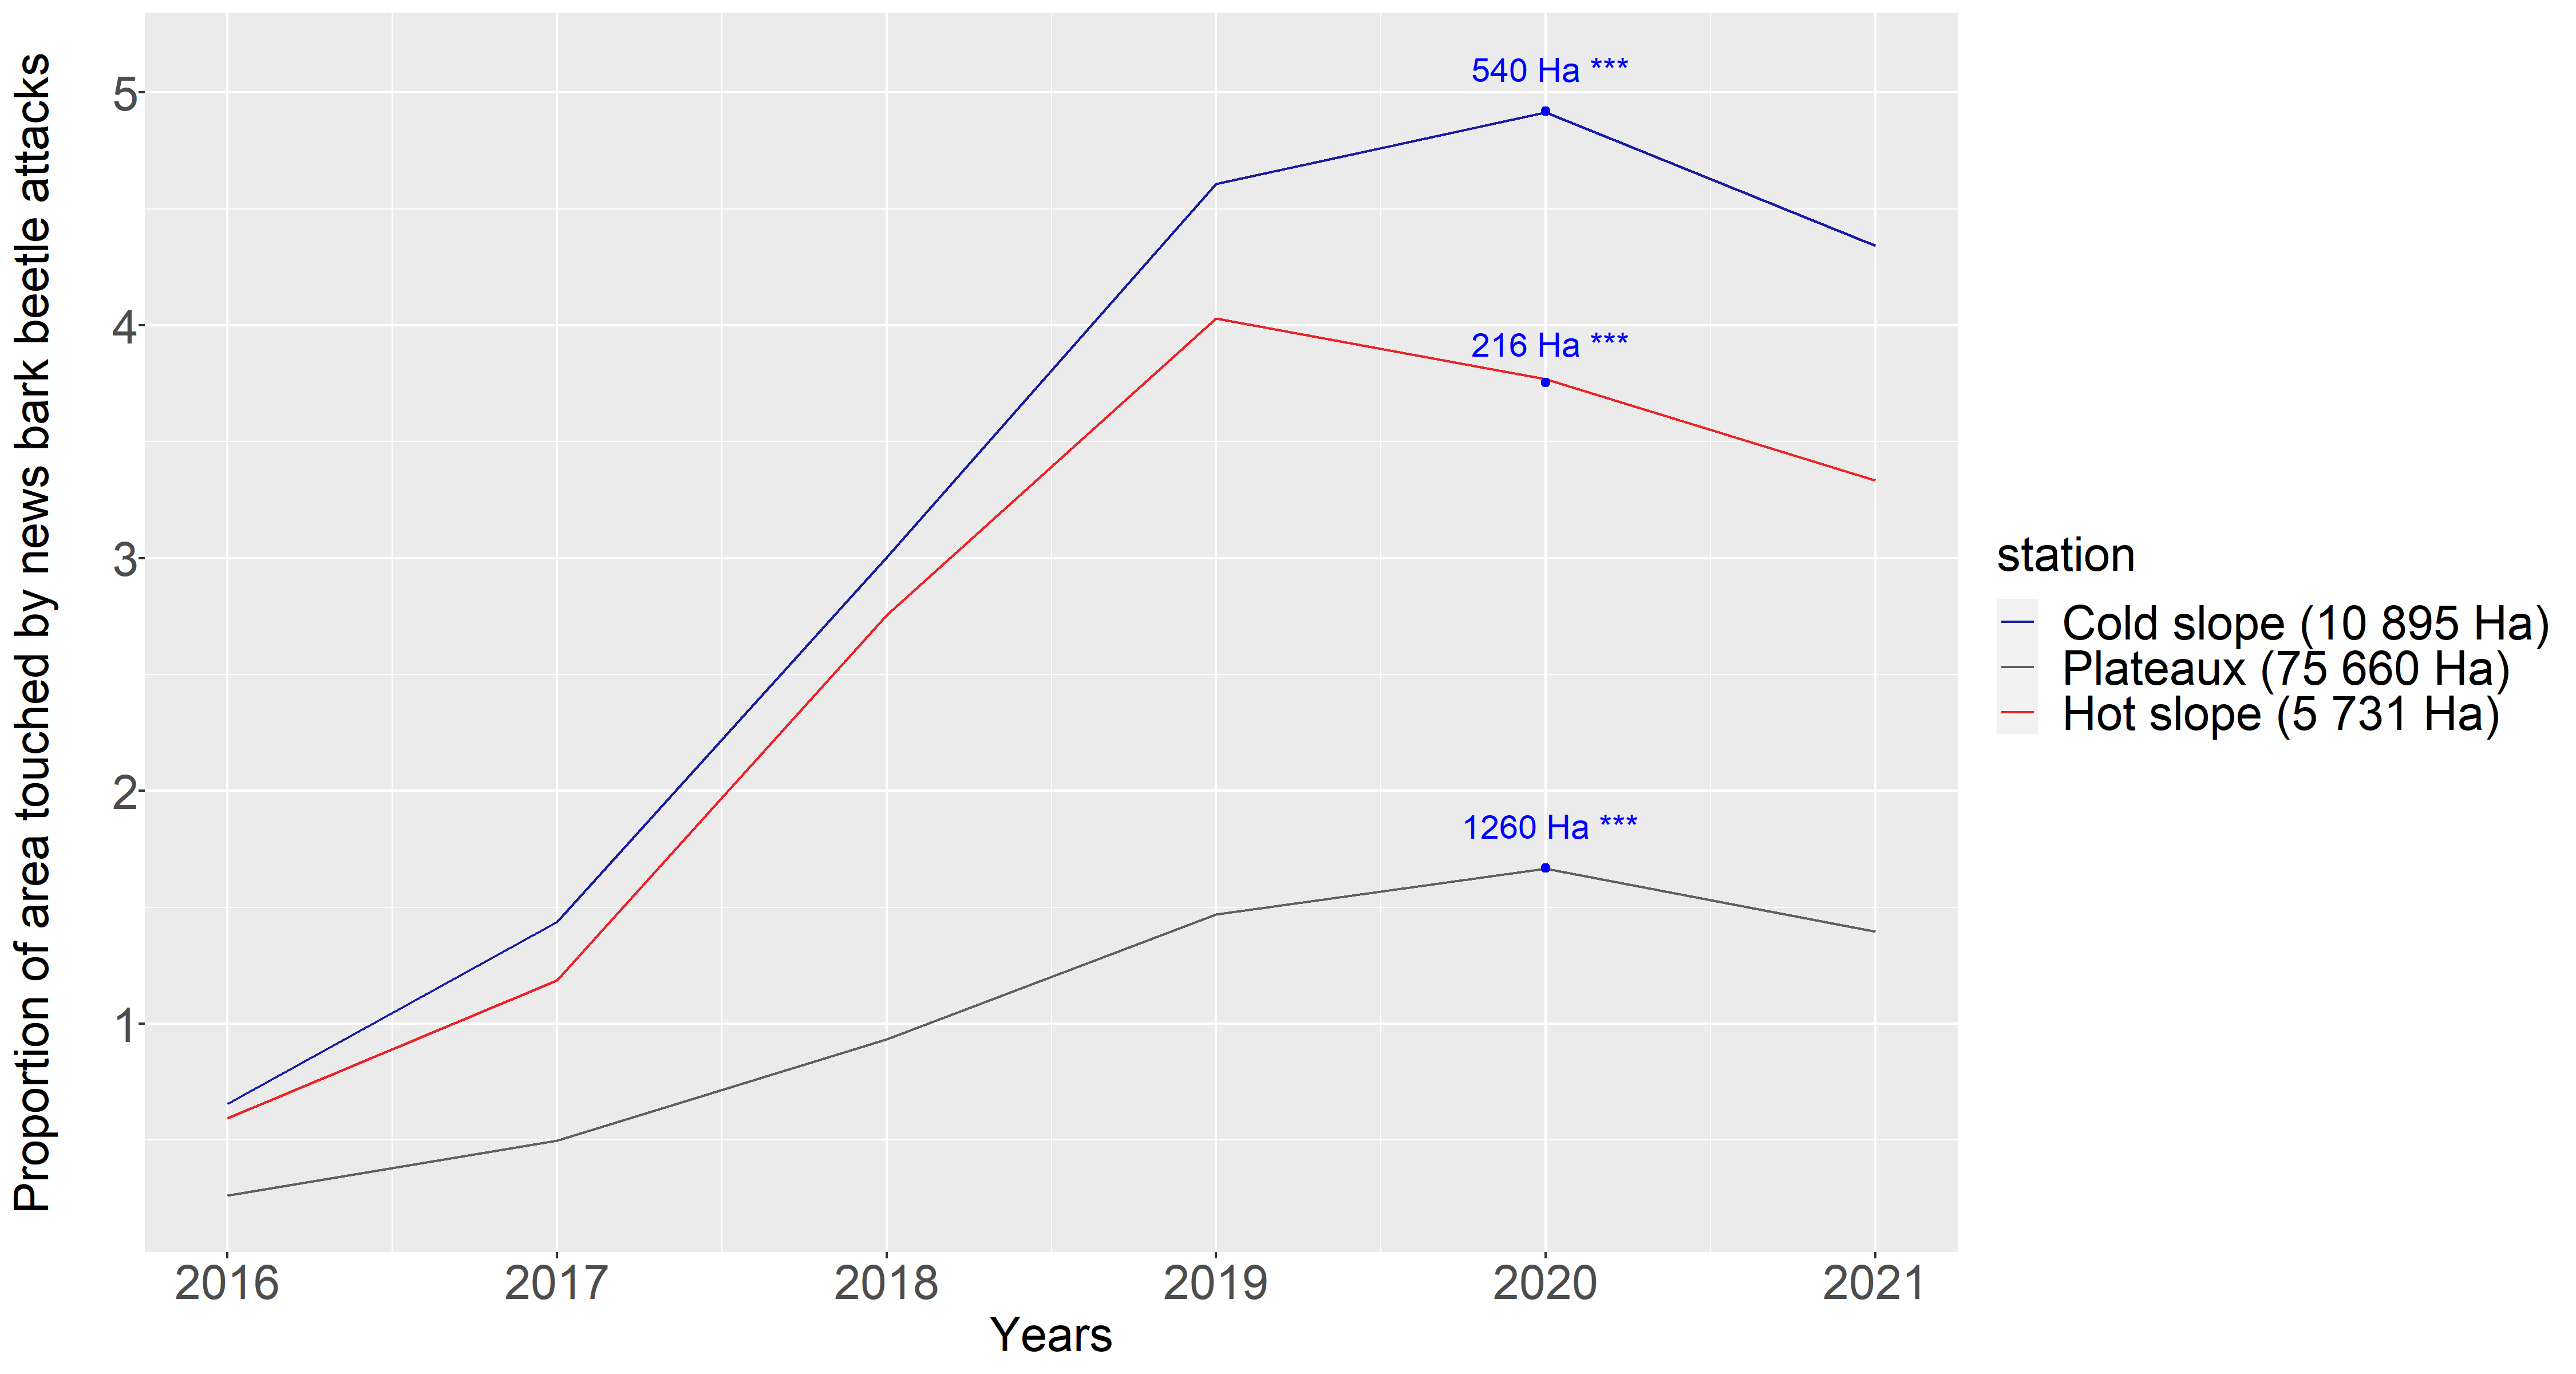
\includegraphics[width=1\textwidth]{evol_ss_wal.png}
		\caption{Évolution de la crise du typographe en région wallonne en fonction des sous-secteurs.}
		\label{fig:ss_wall}
		%\caption sert à insérer une légende
	\end{minipage}\hfill
	\vspace{1cm}
	\begin{minipage}[b]{1 \linewidth}
		\centering
		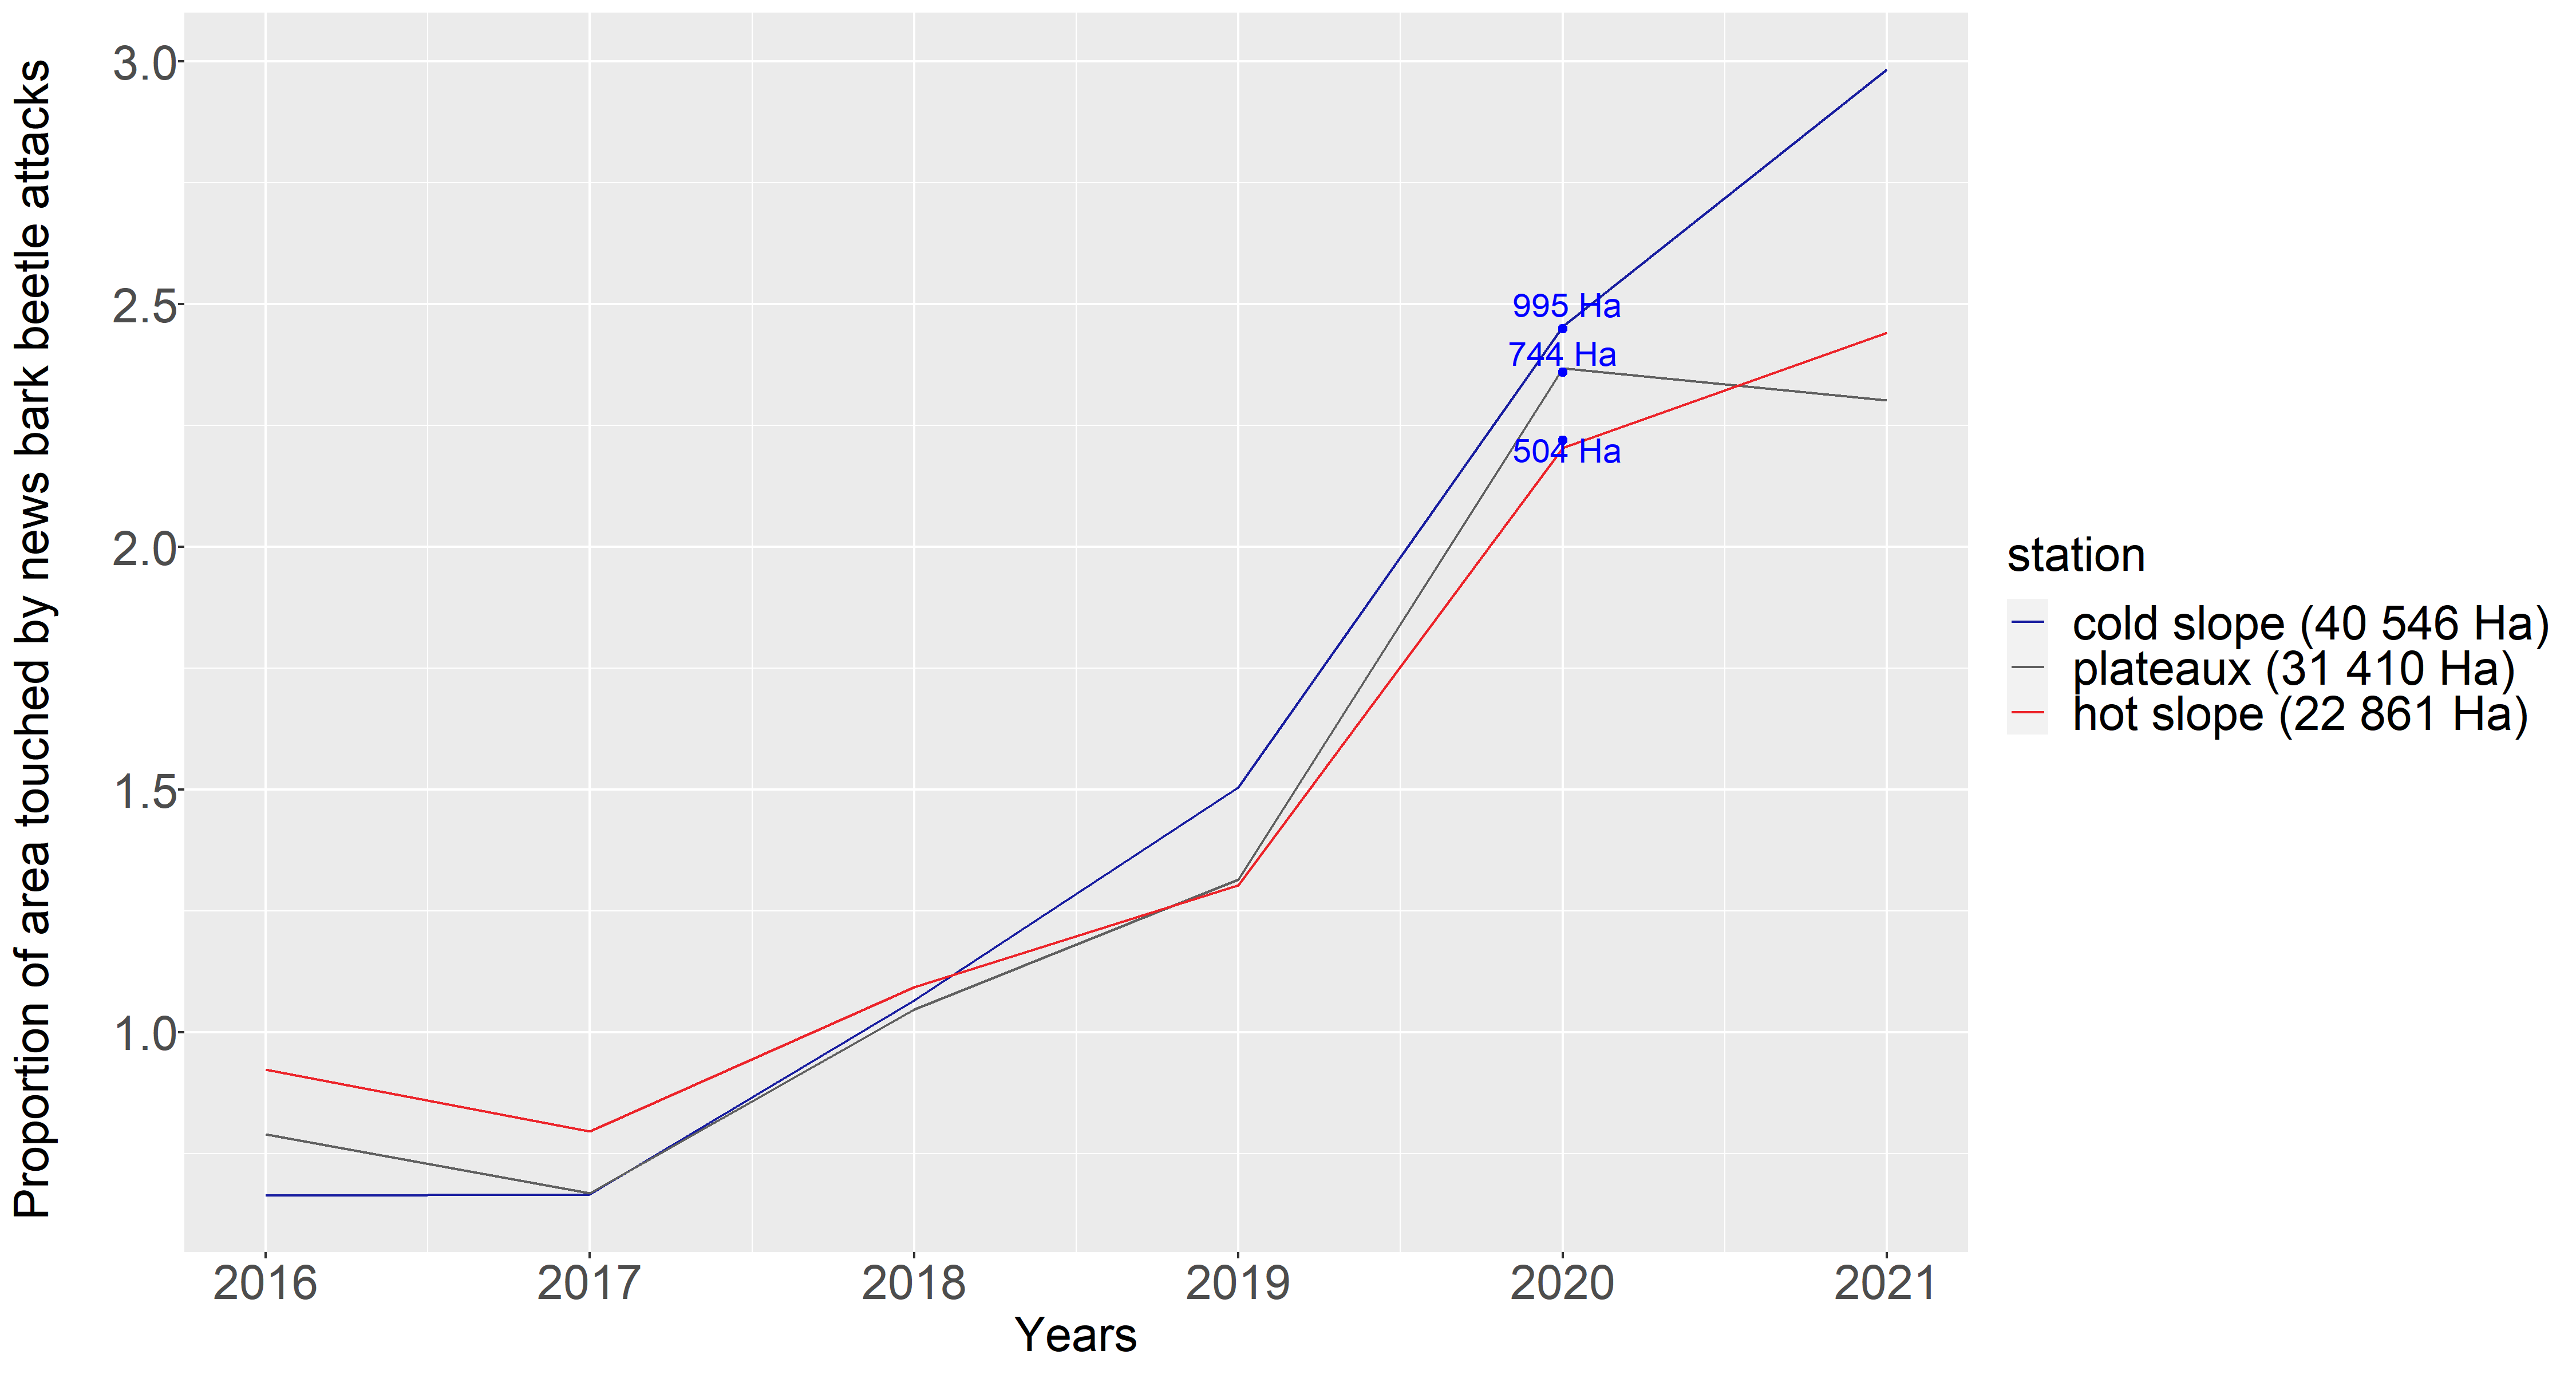
\includegraphics[width=1\textwidth]{evol_ss_vosges.png}
		\caption{Évolution de la crise du typographe dans les Vosges en fonction des sous-secteurs .}
		\label{fig:ss_vosg}
	\end{minipage}
\end{figure}

\section{Acknowledgements}

This research has been funded thanks to the \textit{RegioWood II} project.

\bibliographystyle{elsarticle-num}
%\bibliographystyle{elsarticle-harv}\biboptions{authoryear}
\bibliography{Scolyte.bib}
\end{document}